\documentclass[12pt,a4paper]{article}
\usepackage{cite}
\usepackage{fullpage}
\usepackage{indentfirst}
\usepackage{parskip}
\usepackage{amsmath}
\usepackage{hyperref}
\usepackage{bm}
\usepackage{enumerate}
\usepackage{enumitem}
\usepackage{graphicx}
\usepackage{booktabs}
\usepackage{url}
\usepackage{textcomp}
\usepackage{iitem}
\usepackage{ragged2e}
\usepackage[UTF8]{ctex}

\begin{document}
\justifying
\setlength{\parindent}{2em}

\pdfbookmark[0]{Front page}{label:frontpage}%
\begin{titlepage}
  \noindent%
  \begin{tabular}{@{}p{\textwidth}@{}}
    \toprule[2pt]
    \midrule
    \vspace{0.2cm}\\
    \begin{center}
    \Huge{\textbf{
      基于AODV的支付通道网络\\路由协议 \\[8pt]
    }}
    \end{center}
    \begin{center}
      \Large{
        分布式计算课程主题报告
      }
    \end{center}
    \vspace{0.2cm}\\
    \midrule
    \toprule[2pt]
  \end{tabular}
  \vspace{5 cm}
  \begin{center}
    {\Large
      第15组
    }\\
    \vspace{0.2cm}
    {\Large
      1831605 \quad 刘诗洋 \\[5pt]
      1831606 \quad 陆思远 \\[5pt]
      1831607 \quad 余\quad豪 \\[5pt]
    }
  \end{center}
  \vfill
  \begin{center}
    {\Large
      同济大学\\[5pt]
      软件学院\\[5pt]
    }
  \end{center}
\end{titlepage}
\clearpage

\tableofcontents
\clearpage

\section{概述}
这篇报告是我们以论文\cite{hoenisch2018aodv}为基础,在较为充分的文献查阅及原理探究后,对支付通道网络及其路由协议做的内容梳理。我们从区块链的一大应用:加密货币开始,介绍其现状及共有问题。为了解决这些问题,研究者们提出了链下的支付网络,也即支付通道网络(Payment Channel Network, PCN),其中闪电网络(Lightning Network, LN)是较为突出的代表。但以主动式路由为路由协议的LN存在一些固有局限,为了发挥PCNs的潜力,研究者提出了以AODV(Ad-hoc On-demand Distance Vector)为基础的被动式路由协议,以期有效地解决问题。基于以上问题和解决方案,我们的报告内容也将按这一顺序展开,具体为:
\begin{itemize}
	\item 区块链及其应用的发展、愿景及问题;
	\item 闪电网络;
	\item 支付通道网络的特性、问题及需求;
	\item 路由协议及其种类简介;
	\item 基于AODV的路由协议及算法详述;
	\item 网络及协议性能评价;
	\item 总结与展望。
\end{itemize}

\section{区块链的发展、目标与问题}
随着比特币\cite{nakamoto2008bitcoin}以及其他诸多电子加密货币的出现,区块链一词逐渐被人们所知。作为比特币背后的技术基础,区块链可被认为是所有比特币交易的公共分类账簿\cite{swan2015blockchain}。由于它的去信任化机制,用户可以信任这一系统,并将所有的交易记录在去中心化的节点上;而非像传统做法一样,由中心化的第三方机构来维护。区块链真正的独特技术在于它不需要用户去信任任何的中心机构,而是通过算法的自我监督,任何恶意欺骗系统的企图都将被拒绝。区块链的潜在优势不仅仅体现在金融上,在政府管理、人道主义、社会和科学领域都有可能发挥作用。随着物联网的发展及5G通信时代的到来,机器间的经济交易量也将急剧增长。Gartner\cite{iot_economic}估计,到2020年,全球物联网将包括260亿台设备并产生1.9万亿美元的经济规模。管理这些设备之间的交易需要相应的加密货币,进而形成货币互联网。此外,相互连接的设备之间的小额支付可能会发展成为经济的一个新层次\cite{new_layer_economy}。

区块链旨在建立一个去中心化的网络,然而,随之而来的是一些问题\cite{blockchain_problem}。一个主要问题是,随着区块链网络信息量日益增大,整个网络变得拥挤,交易时间和成本飙升。就比特币来说,一次交易经常需要经过6次区块节点确认,平均耗时超过60分钟;另外,高昂的交易费用也使得小额交易望而却步。除此之外,研究人员发现比特币交易中的数据块可能隐藏着一些非法内容(儿童色情信息等),这些图像或视频文件由于被加密,便与合法的比特币数据混在一起,难以发现。此外,由于比特币的奖励机制,比特币矿工在维护和挖掘比特币时将会得到比特币奖励,但伴随着的是高昂的计算硬件和电力成本。随着维护和挖掘难度增大和比特币的价格变动,成本和收益之间的平衡难以维持,不过目前为止还没有出现网络的崩溃。

针对第一个问题,研究者们设想不在区块链上解决每笔交易,而是将部分交易转移到链下,允许交易双方直接接触。通过自身直接跟踪支付流程,双方即可避免链上交易的高耗时及高费用。若用户存在余额的争议或是有一方无响应,则双方可提供最新的资产负债表并在区块链上解决。在此类解决方案中,闪电网络(Lightning Network, LN)是较为突出的代表,它提出了一个脱链支付通道覆盖网络(PCN),下面我们将详细介绍LN相关内容。


\begin{figure}[htb]
\centering
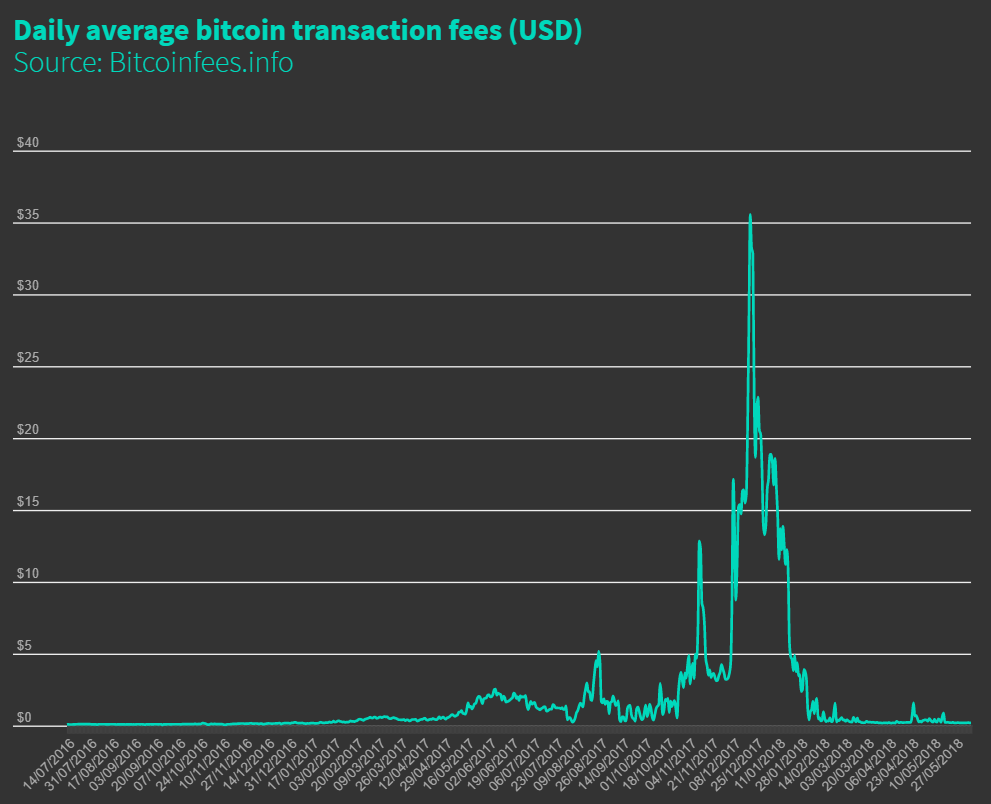
\includegraphics[width=7cm]{fee}
\caption{比特币日均每笔交易费用(美元)}
\end{figure}

\begin{figure}[htb]
\centering
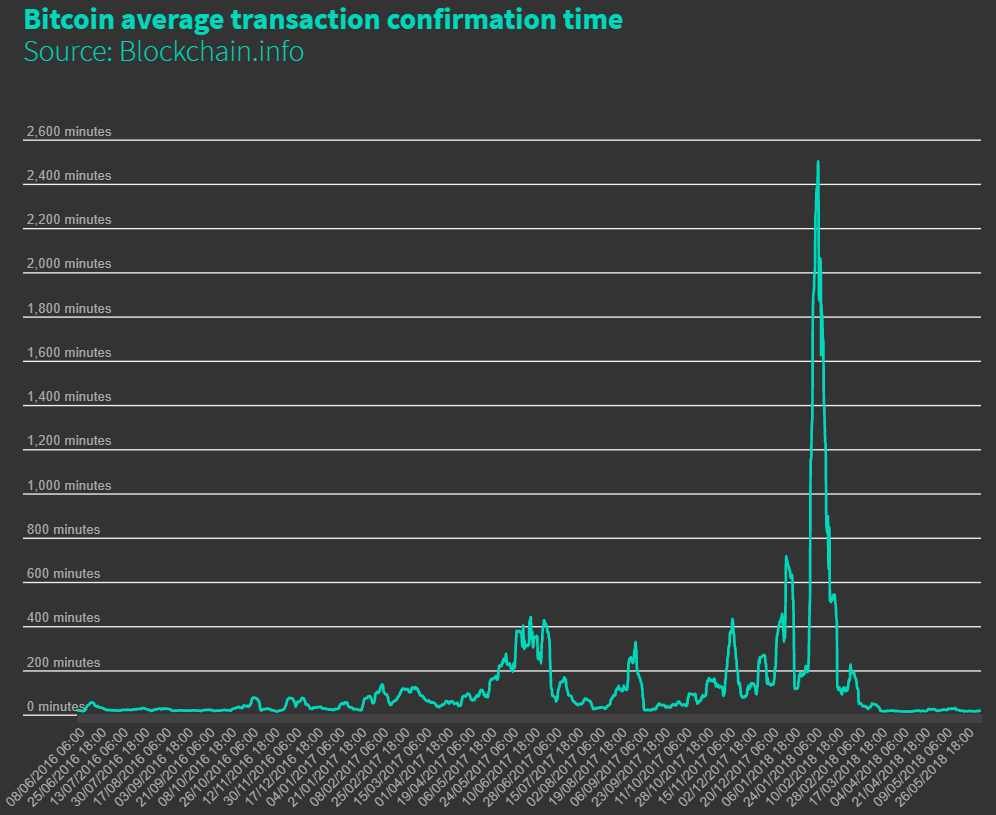
\includegraphics[width=7cm]{time}
\caption{比特币日均每笔交易确认时间(分钟)}
\end{figure}

\clearpage

\section{闪电网络}
\subsection{定义与特性}
闪电网络\cite{poon2016bitcoin}是一种轻量级的软件解决方案,用于扩展公共区块链与加密货币的互操作性。它是一个去中心化的系统,使得即时、大量的小额支付成为可能,且消除了将资金委托给受信任的第三方的风险。闪电网络最初由MIT媒体实验室针对比特币进行研发,但可以拓展应用于所有类似于比特币的区块链。具体来说,闪电网络的功能特性有如下四点。

\begin{enumerate}
	\item 即时支付。比特币将交易聚合成块,每10分钟进行一次。人们普遍认为,比特币在6次区块(耗时约1小时)确认后将被认为是安全的。显然这种确认时间不适合许多场景下的即时交易。而在闪电网络中,支付不需要经由区块确认,可以达到即时性和原子性。因此,闪电网络可以被广泛应用于销售终端、用户设备间交易以及其他需要即时支付的场景。

	\item 小额支付。闪电网络可以使得单笔交易额降至0.00000001比特币(低于0.01美分),且无需承担托管风险,而比特币的链上交易单笔最少数额要比这一值高数百倍。由于比特币单笔交易收费固定(远高于0.01美分),所以在链上进行小额交易是不切实际的。通过闪电网络,小额支付便可以进行,新的市场也得以开辟。


	\item 可扩展性。闪电网络将许多微支付通道连接成为网络,利用这个网络,比特币区块链在一台现代个人电脑上就可每天处理数十亿笔交易。大量的资金可以通过去中心化的方式在给定的交易通道内进行转移,这些通道并非在比特币之上建立独立的信任网络,每一笔经由通道的交易都是真实的比特币交易。

	\item 跨链交易。通过闪电网络,跨链间的原子性交易可以在链下实时发生,只要异构的区块链满足一致性准则。也即只要各个区块链支持相同的哈希函数,就有可能不在受信任的第三方托管下进行跨链交易。
\end{enumerate}

\subsection{关键技术}
闪电网络依赖于区块链的底层技术,通过使用原生的智能契约脚本,并进行真实的比特币交易,就可以创建一个安全的参与者网络,并以高容量和高速度进行交易。下面介绍闪电网络的两个核心概念:RSMC和HTLC。

\textbf{RSMC} (Recoverable Sequence Maturity Contract),即“可撤销的顺序成熟度合同”。首先假定交易双方之间存在一个微支付通道(资金池)。交易双方先预存一部分资金到微支付通道里,初始情况下双方的分配方案等于预存的金额。每次发生交易,需要对交易后产生资金分配结果共同进行确认,同时签字把旧版本的分配方案作废掉。任何一方需要提现时,可以将他手里双方签署过的交易结果写到区块链网络中,从而被确认。从这个过程中可以可以看到,只有在提现时候才需要通过区块链。

任何一个版本的方案都需要经过双方的签名认证才合法。任何一方在任何时候都可以提出提现,提现时需要提供一个双方都签名过的资金分配方案(意味着肯定是某次交易后的结果,被双方确认过,但未必是最新的结果)。在一定时间内,如果另外一方拿出证明表明这个方案其实之前被作废了(非最新的交易结果),则资金罚没给质疑方;否则按照提出方的结果进行分配。罚没机制可以确保了没人会故意拿一个旧的交易结果来提现。另外,即使双方都确认了某次提现,首先提出提现一方的资金到账时间要晚于对方,这就鼓励大家尽量都在链外完成交易。通过 RSMC,可以实现大量中间交易发生在链外。

下面举例说明RSMC的详细过程。假设Alice和Bob需要进行交易,那么在微支付通道建立时,双方必须有一定的资金沉淀在该通道上,我们假设目前通道中资金为:Alice: 0.4,Bob: 0.6,这样预存到通道的资金共有1.0 BTC,其中Alice拥有0.4BTC,Bob拥有0.6BTC。而支付通道的设立会记录在比特币的区块链上。某次,Bob决定向 Alice支付0.1 BTC。在双方都签字认可的情况,链下支付通道的最新余额分配方案将变为{Alice: 0.5,Bob: 0.5},而且双方需要同时签字同意作废前一版本的余额分配方案{Alice: 0.4,Bob: 0.6},这样Alice就实际获得了0.5 BTC的控制权。

若Alice考虑到以后还会和Bob进行交易,那么她可以无需提取现在属于她的0.5BTC,也无需在比特币区块链上更新已有变动的余额分配方案,因为若他们再次进行交易(如Alice向Bob支付0.2BTC)的话,他们仍然只需在链下对目的的余额分配方案达成一致,并设法作废前一版本的余额分配方案就行了。若Alice不打算再次和Bob进行交易并想动用通道的资金,她可以向区块链出示双方签字的余额分配方案。如果在规定时间内Bob未提出异议,区块链则会终止双方的支付通道并将资金按协议转入各自预先设立的提现地址。如果Bob在规定时间内提交证据证明Alice提交的是一个双方已同意作废的余额分配方案,那么Alice的资金将被罚没并给到Bob。

\textbf{HTLC} (Hashed Timelock Contract),即“哈希的带时钟的合约”,用于保证限时转账。通过智能合约,双方约定转账方先冻结一笔钱,并提供一个哈希值,如果在一定时间内有人能提出一个字符串,使得它哈希后的值跟已知值匹配(实际上意味着转账方授权了接收方来提现),则这笔钱转给接收方。

依然使用示例来说明该过程。如图所示,Alice(A)想给Darcy(D)发送0.05 BTC,但Alice和Darcy之间并没有微支付通道。但这没关系,闪电网络为Alice匹配了一条经过Bob(B)、Cady(C)到达Darcy的支付路径,该路径由Alice-Bob,Bob-Cady和Cady-Darcy这样三个微支付通道接力而成。Darcy生成一个哈希值$R$并将$Hash(R)$发送给Alice,Alice不需要知道$R$。$R$和$Hash(R)$的作用类似于钥匙和锁,只有匹配在一起才可开锁。Alice和Bob商定一个HTLC合约:只要Bob能在3天内向Alice出示正确的$R$,Alice会支付Bob 0.052 BTC;如果Bob做不到这点,这笔钱3天后自动退还Alice。同样地,Bob和 Cady商定一个HTLC合约:只要Cady能在2天内向Bob出示哈希正确的$R$,Bob会支付 Cady 0.051 BTC;如果Cady做不到这点,这笔钱到期自动退还Bob。最后,Cady和 Darcy商定一个HTLC合约:只要Darcy能在1天内向Cady出示哈希正确的$R$,Cady会支付Darcy 0.05 BTC;如果Darcy做不到这点,这笔钱到期自动退还Cady。

方案确定好后,Darcy及时向Cady披露$R$并拿到0.05 BTC;现在Cady知道了$R$,她可以向Bob出示密码$R$并拿到0.051BTC(差额部分的0.001 BTC成了Cady的佣金);Bob 知道$R$后当然会向Alice出示并拿到他的那份 0.052 BTC,差额部分的 0.001 BTC成了Bob的佣金。大家可以看到,最终的结果是Alice通过闪电网络安全地向Darcy支付了 0.05 BTC,所付出的代价仅仅是支付给Bob和Cady(节点)的 0.002 BTC“过路费”(佣金)。

\begin{figure}[htb]
\centering
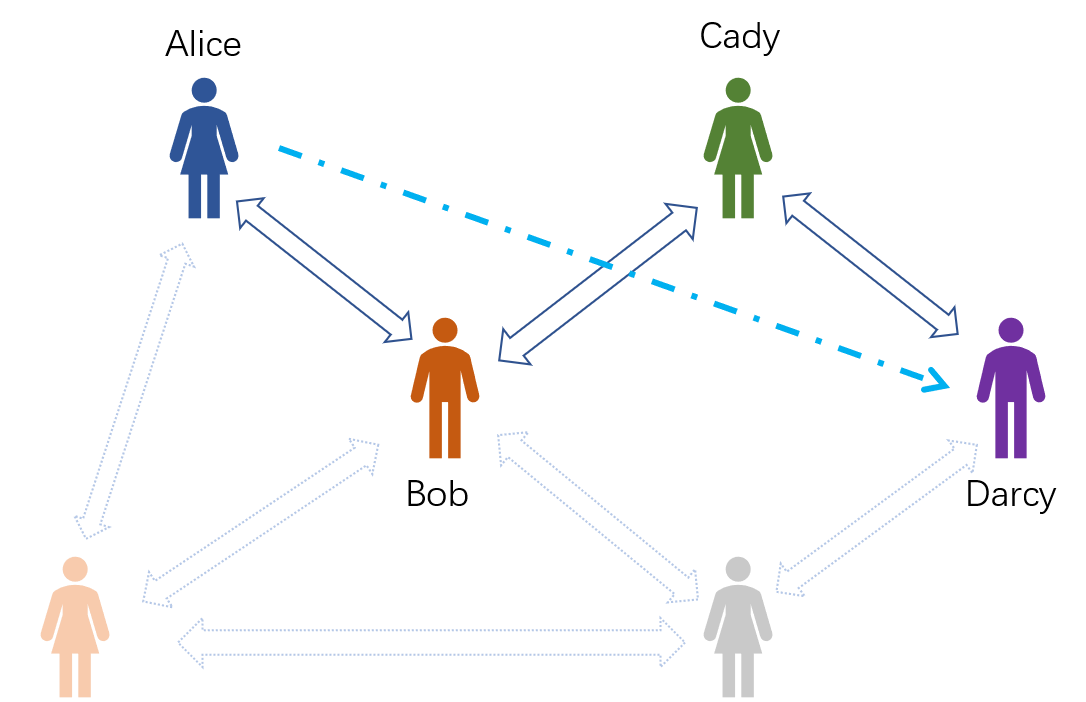
\includegraphics[width=9cm]{channels}
\caption{闪电网络微支付通道}
\end{figure}

\subsection{小结}
闪电网络的理念就是引入了一个类似于第三方中介且仅适用于高频次、小额交易的微支付通道。交易双方在这个微通道中必须先预存一定数量的保证金,而由区块链产生的智能合约(资金分配方案)进行监督评判。闪电网络中的所有交易动作都是发生在区块链之外,只有当需要提现时,才会将最终的交易结果写到区块链网络中并被最终确认。这大大降低了比特币区块链上的交易压力。

其中,RSMC 保障了两个人之间的直接交易可以在链下完成,HTLC 保障了任意两个人之间的转账都可以通过一条“支付”通道来完成。闪电网络整合这两种机制,就可以实现任意两个人之间的交易都在链下完成了。智能合约起到了中介的重要角色,而区块链网络则确保最终的交易结果被确认。

\section{PCN路由协议}

\subsection{PCN的通道寻优}
如第三部分所述,当交易双方之间没有直连的微支付通道时,需要将若干个支付通道连接,方可进行交易。在这个过程中,如何在发送方和接收方之间寻找到最优(或可接受)的路由通道将是一个挑战。在这个特定网络里,路由协议需要考虑路由费用、汇率以及可靠性等指标,使之可被接受。闪电网络使用主动式的路由协议,每个节点通过网络广播其邻居的信息(例如,广播通过网络连接的节点信息)。每个节点都具有关于网络拓扑的路由表,然而,这样做的缺点是在建立路由前需要发送大量信息。而且,在这样的基础上,我们只能获知通道的金融信息,而不包括整个资金的分布,也即想要获知哪一方拥有多少金额,只能寻求与比特币的区块链。显然,广播全局的拓扑信息耗费巨大,且会产生扩展限制,这在跨链网络的情况下尤为严重。因此,研究者们寻求设计其他路由算法,以求突破这一限制,下面先简要介绍主要的几种路由协议。

\subsection{PCN的基本假设}
在针对PCN提出路由算法前,先提出对PCN的基本假设:网络处于持续变化(网络的变化发生得比节点发出支付操作更频繁)。网络的持续变化源自于以下几个情况:
\begin{enumerate}
	\item 通道频繁更改:如付款前有效的路由在付款后不一定有效。
	\item 费用可能会经常变动:每个中间节点在转发支付时可以收取任意数量的费用。该节点可以定期更新该费用,以保持其通道平衡。例如,如果一个通道的流动性有耗尽的风险,节点在通过该通道转送付款时可能会收取更高的费用。
	\item 汇率可能变化很快:两个区块链之间的节点需要频繁地调整汇率;否则,这个节点可能有赔钱的风险。
	\item 节点可能在一段时间内处于脱机状态(或不可到达状态):
	由于在支付过程中节点需要接受和转发支付请求,所以节点基本是随时在线的,但如果中间节点离线,网络应该相应地进行调整。
\end{enumerate}

\subsection{路由协议的类型}
路由指电子通信网络通过确定网络中的路径,并通过这种路径高效快速地将一个信息单元从A点发送到B点的能力\cite{medhi2017network}。而路由协议则是描述具体的寻路算法,使得整个网络通信更加高效且可靠。由于目前研究者对PCN的研究较少,所以我们将目光移向移动自主网络(MANET, Mobile Ad hoc Network)。MANET是指能够自主配置的可移动节点的网络集合,集合内的节点可以自由移动,并可在任何时候连接到不同的节点。与PCN类似,MANET内的节点的出现和消失并不规律,且通道的平衡经常变化。在MANET里,路由协议可以分为五大类型:主动协议、被动协议、混合协议、分层协议和基于协调的协议。

主动协议\cite{Alslaim2014}使用链路状态路由算法,每个节点都会维护一到多个包含路由到网络中其他所有节点的路由表。所有的节点持续更新它们的路由表来维护最新的网络视图。这种路由协议适用于静态场景,两个较为著名的协议为DSDV(Destination-Sequenced Distance Vector routing)和WRP(Wireless Routing Protocol)\cite{Murthy1996}。

被动协议减少了主动协议中存在的开销。它使用距离向量路由算法,并且仅当一个节点启动路由发现过程请求指定目的地时,才建立到该目的地的路由。在信息到达目的地后,以及这条路由不再需要前,该路由持续有效。比较典型的协议有AODV(Ad-hoc On-demand Distance Vector)和DSR(Dynamic Source Routing)\cite{Johnson, Perkins1999}。

混合协议将主动协议与被动协议混合,在此种协议下,每个节点主动维护一定区域内的路由信息表,若目的地超出了这一范围,则使用路由发现过程。混合协议的代表有ZRP(Zone Routing Protocol)、EIGRP(Enhanced Interior Gateway Routing Protocol)。

表格\ref{protocols}比较了上述三类协议的异同。

\begin{table}[htb]
\renewcommand\arraystretch{1.2}
\caption{主动协议、被动协议与混合协议异同比较}
\centering
\begin{tabular}{l l l l}
\label{protocols}
\\
\hline
\hline
~ \textbf{特征} ~ & ~ \textbf{被动协议} ~ & ~ \textbf{主动协议} ~ & ~ \textbf{混合协议} \\[6pt]
\hline
路由结构  & 扁平结构 & 扁平及分层结构 & 分层结构 \\[6pt]
\hline
路由获得 & 按需获取 & 表驱动 & 二者混合
\\[6pt]
\hline
路由开销 & 低 & 高 & 中等
\\[6pt]
\hline
延迟 & 高(由于泛洪) & 低(由于主动路由) & 中等
\\[6pt]
\hline
可扩展性 & 不适用于大型网络 & 低 & 适用于大型网络
\\[6pt]
\hline
路由信息 & 需要时可用 & 始终可用 & 介于二者间
\\[6pt]
\hline
定期更新 & 不需要 & 网络改变时即需更新 & 需要
\\[6pt]
\hline
移动性 & 路径维护 & 定期更新 & 二者结合
\\[6pt]
\hline
存储需求 & 低 & 高 & 中
\\[6pt]
\hline
带宽需求 & 低 & 高 & 中
\\[6pt]
\hline
电力需求 & 低 & 高 & 中
\\[6pt]
\hline
\hline
\end{tabular}
\end{table}

而分层路由和基于协作路由的协议是通过位置相关的地址来进行路由的,用基于位置的算法取代了泛洪传播消息。前者的典型例子有LANMAR\cite{Guangyu}和L+\cite{mitton2005distributed},后者的例子有GPSR\cite{Karp2000}和BVR\cite{fonseca2005beacon}。

上述路由协议大多数都是为MANET设计,与PCN的需求还有些不同。例如,由于PCN涉及到资金锁定、汇率变动、节点费用变动等,一个路由响应会改变网络的状态,使得先前的通道不可用。但研究者们依然可以从MANET路由协议中获取一些灵感。

\clearpage

\subsection{Flare协议}
Prihodko等人提出了针对闪电网络的路由协议Flare\cite{prihodko2016flare}。Flare协议作为混合式协议,由主动和被动两个部分,提出该协议主要基于闪电网络的信息可以被分为两类:
\begin{itemize}
	\item 缓慢变化或静态的信息(节点之间的支付通道);
	\item 快速变化或动态的信息(节点状态、支付通道内资金分配、使用通道费用等)。
\end{itemize}

因此,主动(按确定的时间周期或按受限的泛洪方式)收集闪电网络中刚打开或关闭的支付通道是有意义的,这部分信息是闪电网络节点的兴趣内容;而主动收集会快速变化的信息是没有意义的,因为它们在不可预测的时间内都可能发生改变。

下图是Flare协议算法的概要架构。图中路由模块对应的便是闪电网络的业务逻辑。该模块的目标是提供一个或多个支付路径(如LN节点列表)发送给指定的收件人。为了实现这一目标,节点点通过交互来获取网络信息。获取方式包括主动(通过发现节点的邻居和信标)以及被动(通过选择和排序候选路线)。收集到的信息被放置到节点的路由表中,路由表用于处理来自节点操作者和其他节点的请求。

\begin{figure}[htb]
\centering
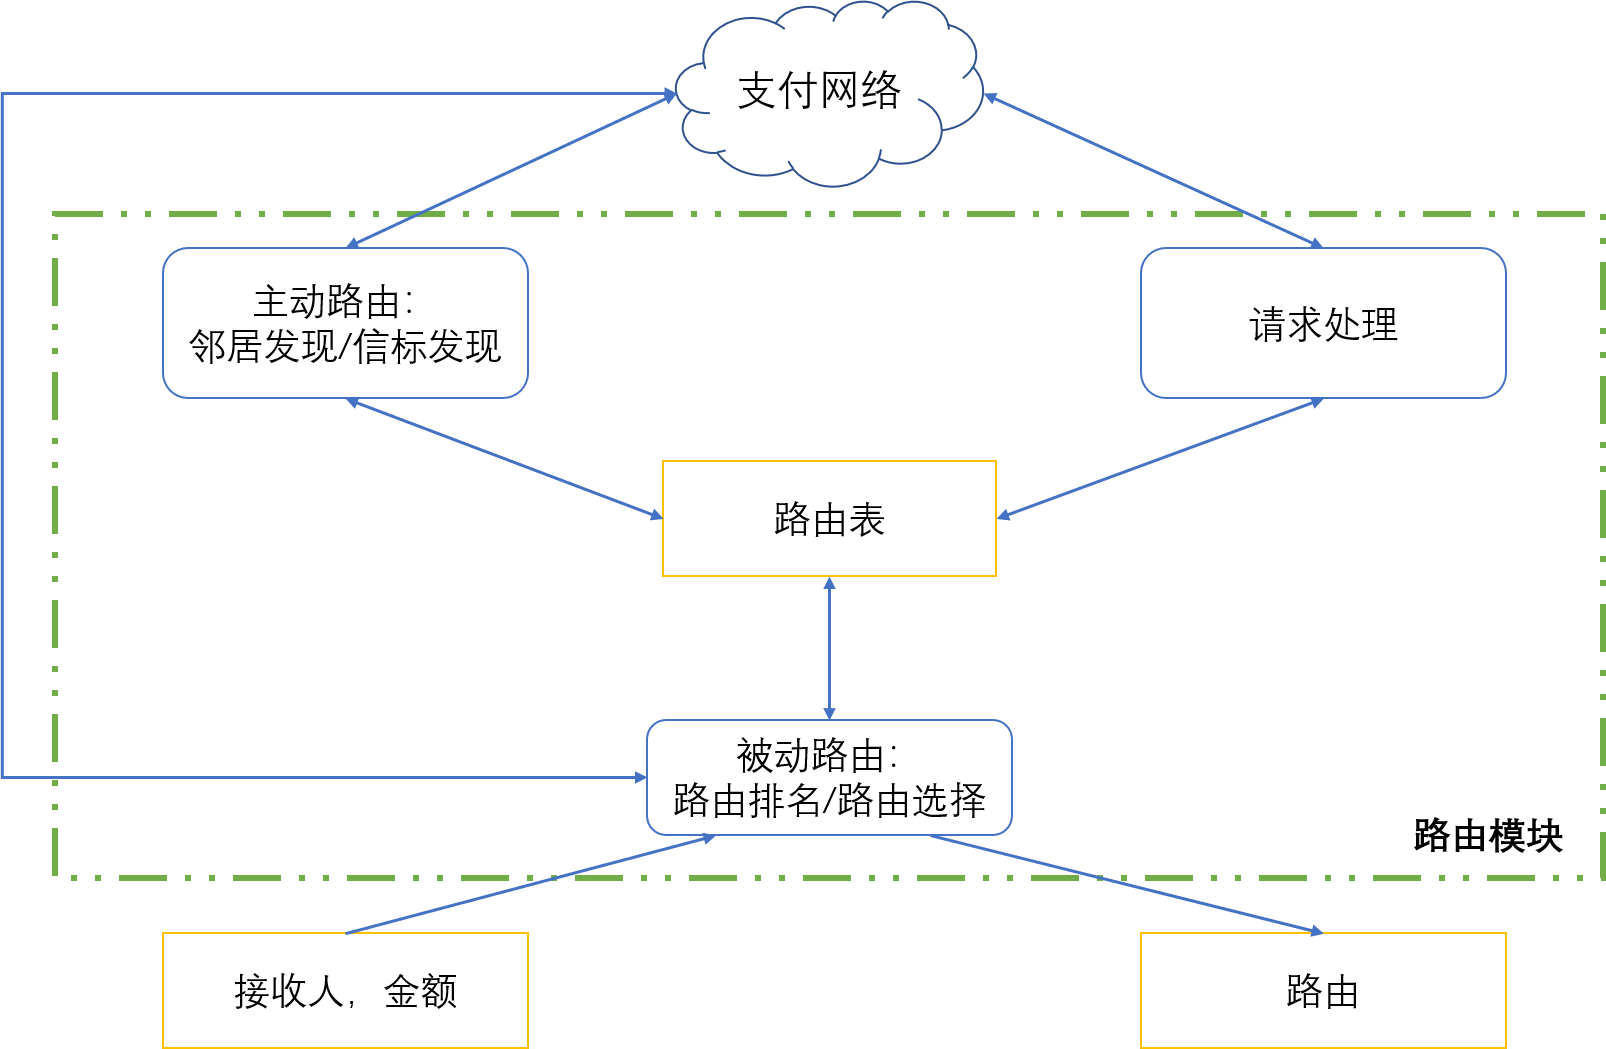
\includegraphics[width=12cm]{high_level_flare}
\caption{Flare协议抽象架构}
\end{figure}

与Flare不同,Hoenisch等人提出了另一种解决方案\cite{hoenisch2018aodv}。他们认为Flare专注于发送节点的安全性和审查阻力,而\cite{hoenisch2018aodv}关注每个中间节点的自主性。每个节点不应被迫将支付转发到某个特定的方向,这个决策是从经济的角度出发的。他们假设节点主要关注利润最大化,因此更有可能选择保证高利润的路线。这一基于AODV协议的算法是本篇报告所要阐述的重点,将在下文展开。

\subsection{PCN的路由需求与算法选择}
为了高效、经济、可靠地进行加密货币交易,一个合适的路由算法是至关重要的。电子货币的社区提出了若干愿景\cite{beliefs},或称为对网络的要求,这些要求可以作为设计可行的路由算法的参考依据。

\begin{enumerate}
	\item 自洽与自立(Autonomy and self-reliance)。为了提供高可用性和抗故障网络,节点需要是自配置的,即每个节点应该能够独立自主地工作。因此,节点应该能够同时充当发送方和接收方,并且应该能够将支付请求路由到任何方向。此外,尽管网络拓扑结构发生了随机变化,或者某些节点的行为错综复杂,但网络的功能必须得到保留。

	\item 成本保证(Cost guaranties)。支付通道网络中的每个节点都可以收取一定的费用(佣金)来转发支付。此外,当跨越不同区块链时,桥接节点将指定两种货币之间的特定汇率。因此,至关重要的是,在执行付款之前,必须知道从发送方到最终接收方的整个网络支付的总成本:因为发送方希望确保所需的金额到达最终接收方,而不是被费用或汇率吞噬。

	\item 时间锁定保证(Time-lock guaranties)。该网路需要为每次付款行为(通道更新)分配一个时间锁。这有两个目的:第一,接收方需要足够的时间来赎回支付;第二,发送方需要足够的时间在发生故障时回滚。

	\item 弹性(Flexibility)。路由协议需要足够的灵活,以应对流量变化。在一个庞大的网络中,变化可能发生在各个方面:支付通道可能出现或消失;通道的资金分配可能发生变化;节点可能更新费用(佣金);区块链之间的节点可能改变汇率,以避免亏损。

	\item 阻止网络分割(Prevent network partitioning)。单个(或多个)失败节点不应预先阻止支付路由或将网络分割为子网络。一个节点应该总是能够找到一个路径,通往接收方,即没有其他节点能够阻止支付。换句话说,如果一个路由存在于两个节点之间,路由协议应该能够找到它。

	\item 实时性(Real-time)。PCN的一个主要目标是实现即时小额支付,因此实时性是该网络的基本能力保证。网络流量延迟是唯一允许的时间限制,路由时间应该少于几秒钟。

	\item 信息同步保证(Up-to-dateness)。拥有最新的可用信息对于通过网络找到最佳路径至关重要。因此,该网络要求通过路由协议找到的路由包含有关费用和汇率的最新信息。

	\item 轻量、可扩展(Lightweight and scalable)。随着时间的推移,预计支付通道网络的规模将会持续增长。因此,路由应该能够适应它,并与之伸缩。此外,路由应该只使用一定量的资源,而非无限扩张。

	\item 去信任化(Trustlessness)。当节点发生拜占庭行为(即在费用或路由方面进行欺骗)时,路由应该经得起考验。

	\item 寻求每个节点的最佳方案(Optimal solution for each node)。路由协议应该允许每个节点在其自身的经济激励下行动。这种激励因节点而异,例如,发出支付的节点可能希望沿着最便宜、最快或成功率最高的路径发送支付。另外,如果某个转发行为损害了节点自身利益,那么它有权不予转发。
\end{enumerate}

\subsection{小结}
本节重点关注支付通道网络的路由协议,先指出PCN路由的重要性以及LN中路由算法的局限性,再提出PCN的基本假设(持续变化性),通过梳理与类似PCN的MANET 网络路由协议类型来寻求合适于支付通道网络的路由算法。同时,我们也关注了现有的专注于PCN的网络协议:Flare,分析其机理以及局限性。最后,我们总结了电子货币社区对支付网络的若干愿景及目标,以作为设计合适的协议的参考依据。

\section{AODV协议}

\subsection{定义}
无线自组网按需平面距离向量路由协议(Ad hoc On-Demand Distance Vector Routing,AODV)是应用于无线随意网络(无线Ad hoc网络)中进行路由选择的路由协议,它能够实现单播和多播路由\cite{Perkins2003}。该协议是Ad Hoc网络中按需生成路由方式的典型协议。AODV是最初为MANET\cite{cs441_manet}(快速移动自组网)和其他无线自组网设计的路由协议设计的,同样也是应用最广泛的按需路由协议之一。

\subsection{AODV的特性}
AODV是反应式路由协议,即需要向目的节点发送包时,源节点才在网络中发起路由查找过程,找到相应的路由。AODV协议是DSDV算法的改进,但中间节点不需要事先维护路由。AODV具有以下特性:
\begin{itemize}
	\item 适用于有大量节点的无线自主网络;
	\item 能够快速适应动态条件变化;
	\item 较低的处理和内存开销;
	\item 路径无环;
	\item 路由是在逐跳的基础上根据需要建立的;
	\item 通信过程是对称的,路由可逆。
\end{itemize}

\subsection{AODV与先验式协议的比较}
大多数网络路由协议都是先验式的,即查找路由的过程并不依赖于路径上的节点是否要发包,而是每个节点各自维护一张包含到达其它节点的路由信息的路由表。节点间通过周期性的交换路由信息来不断更新自身的路由表,以便能够及时的反映网络拓扑结构和变化,以维护一致的、及时的、准确的路由信息。

\subsection{AODV与Flare的比较}
% 此处需讨论,修改
Flare算法是基于源路由的主动路由算法。与AODV不同,源路由可以很容易地与Onion路由结合,为网络参与者带来更高级别的安全性。它允许在不同的层中加密支付消息,这样中间的节点就不会知道消息的最终目的地是什么,或者最初的发送方是谁。然而,缺点是发送节点可以间接攻击中间的任意节点,如通过抽干它的流动性从而锁定一段时间,这样它就不能再继续支付了;更糟糕的是,如果消息被加密,被攻击的节点甚至根本不知道它从哪里受到攻击。

\subsection{AODV协议分析}
AODV路由协议\cite{cs647_aodv}是一种典型的按需驱动路由协议,该算法可被称为纯粹的需求路由获取系统,那些不在活跃路径上的节点不会维持任何相关路由信息,也不会参与任何周期路由表的交换。此外,节点没有必要去发现和维持到另一节点的路由,除非这两个节点需要进行通信。

AODV算法旨在多个移动节点中建立和维护一个动态的,自启动的,多跳路由的专属网络。AODV使得移动节点能快速获得通向新的目的节点的路由,并且节点仅需要维护通向它信号所及范围内的节点的路由,更远的节点的路由信息则不需要维护。网络中连接的断开和异动会使得网络拓扑结构发生变化,AODV使得移动节点能适时对这种变化做出响应。

\subsubsection{AODV的节点计数器}
AODV协议中,每个节点都要维护两个计数器:

\begin{itemize}
	\item 节点序列号
	\item 广播ID:只有当发出一个新的REQ的时候才会更新
\end{itemize}

\subsubsection{AODV的消息种类}
\begin{itemize}
	\item 路由请求(RREQ)
	\item 路由回复(RREP)
	\item 路由错误(RERR)
\end{itemize}
当活动路由表里有一条连接断开时,一条RERR消息(路由错误消息)将被用来通知其他节点发生了连接断裂。RERR消息指出了不再能到达的目的节点(甚至是目的子网)。

\subsubsection{AODV路由表}
AODV路由表每项只记录下一跳路由信息,而不是整条路由的信息,简化了路由表的建立和维护。AODV中每一个节点所维护的路由表的主要字段:
\begin{itemize}
	\item 目的节点的IP地址
	\item 目的节点的序列号
	\item 目的节点的有效标志位
	\item 下一跳节点对应的IP地址
	\item 本节点到达目的节点的跳数
	\item 前驱节点列表
	\item 有效时间(路由失效或删除时间)
\end{itemize}

\subsubsection{AODV的关键}
为了维持节点间的最新路由信息,AODV协议借鉴了DSDV中的序列号的思想,序列号可以用来反映此路由的新鲜度,一般序列号越大,路由越新鲜,这是保证开环的重要措施,在路由发现和路由回复,更新路由时均需要进行序列号的比较。源节点和目的节点都需要维护自己的序列号,于是如何管理序列号是提高路由建立和维护的关键。

AODV要求每一个节点的每一个路由表项必须包含关于目的节点IP地址的序列号的最新可用信息,这个序列号叫做“目的序列号”。目的序列号由目的节点创建,并且被包含在路由信息中,然后这些路由信息将被回发到所有向它发起请求的节点,以保证朝向这个目的节点的所有路由路径都是无环路、无回环的。如果在任何时候一个节点接收到了新的信息,而这个信息是跟RREQ,RREP,或者RERR消息中的序列号有关的话,目的序列号就会更新。(即如果到一个目的有两条路由可供选择,那么收到请求的节点将会选择序列号最大的那一条)。

在两种情况下,目的节点会增加它自己的序列号:
\begin{itemize}
	\item 在一个节点发起一个路由发现的请求之前,必须增加它自己的序列号。这样,对于已经建立好了的朝向RREQ消息发起者的反向路由来说,可以防止本次请求与其相冲突。
	\item 在目的节点生成RREP消息以响应RREQ消息之前,它必须更新它自己的序列号,新的值是它目前的序列号和RREQ消息包中目的序列号的较大者
\end{itemize}

另外,节点为了修复路由路径中丢失了的或者过期了的下一跳时,可能会改变其路由表项中的目的序列号,这也是除了以上情况以外唯一要改变目的序列号的情况。节点通过查询其路由表来查询都有哪些目的节点使用了这个不可使用的下一跳节点。在这种情况下,对于每一个使用这个节点的目的节点,当前节点都会增加其序列号并把此路径标记为不可用。一旦节点接收到了一个足够新的(也就是包含大于等于本节点所记录的序号),并且是来自于已经标记相应路由表项为不可用的节点的路由信息时,当前节点应该以新的信息来更新其路由表信息。

\subsubsection{AODV消息的重要字段(域)}
\begin{itemize}
	\item Destination Sequence Number(目标节点序列号)。发起节点在以前通往目标节点的路由信息中能找到的最新的序列号
	\item RREQ ID(路由请求标识)。这是一个序列号,用它和发起节点的IP就可以唯一标识一个RREQ信息。
	\item Originator Sequence Number(发起节点序列号)。指向发起者的路由表项中正在使用的序列号
	\item Hop Count(跳数)。从发起节点到目标节点的跳数。对多播路由请求,这个跳数则是从发起节点到多播节点组里产生RREP信息的节点的跳数。
\end{itemize}

\subsection{AODV路由建立和数据传输过程}
\subsubsection{生成路由请求}
当一个节点无法找到到达某个节点的路由时(可能由于路由表中并不存在这样一个目的节点,抑或者是到达该目的节点的有效路由过期,或被标记为无效),它就会广播一条RREQ消息。

在RREQ中主要包含如下内容:

\begin{itemize}
	\item 源节点序列号:用于维持到源节点的反向路由的特性,在把它放入RREQ消息里时,需要先自增1。
	\item 源节点所知道的最新的目的序列号:表明了到目的节点的最新路由;该序列号直接就从路由表里的“Destination Sequence Number”域复制过去。如果尚未获得任何目的节点序列号,则“序列号未知”标志必须被置位。
	\item RREQ ID:将当前节点以前用过的RREQ ID加一,每个节点只维护一个RREQ ID。
	\item Hop Count:置为0。
\end{itemize}

在广播RREQ消息之前,发起节点会将消息的RREQ ID和Originator IP address缓存一段时间,这个时间由“PATH\_DISCOVERY\_TIME”来决定。这样,当这个节点从邻居那里收到具有相同RREQ ID和Originator IP address的RREQ消息时,它将会认为这是一个发回来的包而将它丢弃。

\begin{figure}[htb]
\centering
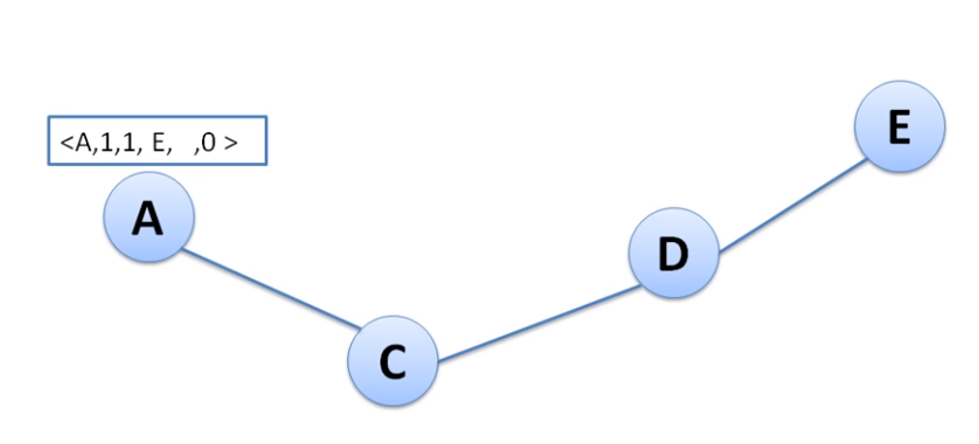
\includegraphics[width=9cm]{gen_route_request}
\caption{生成路由请求}
\end{figure}

\subsubsection{处理和转发路由请求}
一个发起节点总是想和目的节点建立双向的通信,即仅仅是有发起节点有到目的节点的路由还不够,目的节点还必须拥有回到发起节点的路由。因而当RREQ从一个源节点转发到不同的目的节点时,沿途所经过的节点都要自动建立到源节点的反向路由。

节点通过记录收到的第一个RREQ的邻居节点的地址来建立反向路由,或更新原有路由(即更新反向路由表),这些反向路由将会维持一定时间,该段时间足够RREQ在网络内进行转发以及产生的RREP返回源节点。

同时会检查在PATH\_DISCOVERY\_TIME时间内是否受到过具有相同Originator IP Address和RREQ ID的RREQ消息。如果已经接收过了,那么这个节点就会丢弃这个 RREQ,不作任何操作。当RREQ到达了目的节点,目的节点就会产生RREP,并利用建立的反向路由来转发RREP。

在转发RREQ前,需要对其进行更新,RREQ消息内的跳数会加一,表明该RREQ 又跳过了一个中间节点;Originator Sequence Number(发起节点序列号)会被用来和反向路由里对应的目的节点序列号比较,如果比已经在路由表里的那个大,那么就会被复制到路由表里面。

\begin{figure}[htb]
\centering
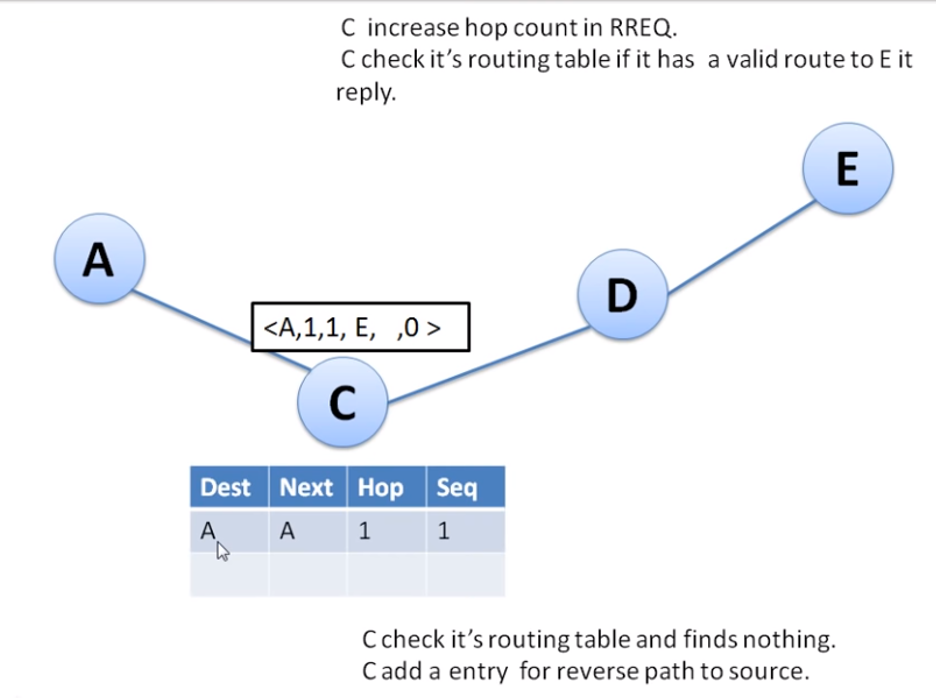
\includegraphics[width=8cm]{handle_route_request_1}
\caption{处理和转发路由请求:1}
\end{figure}

\begin{figure}[htb]
\centering
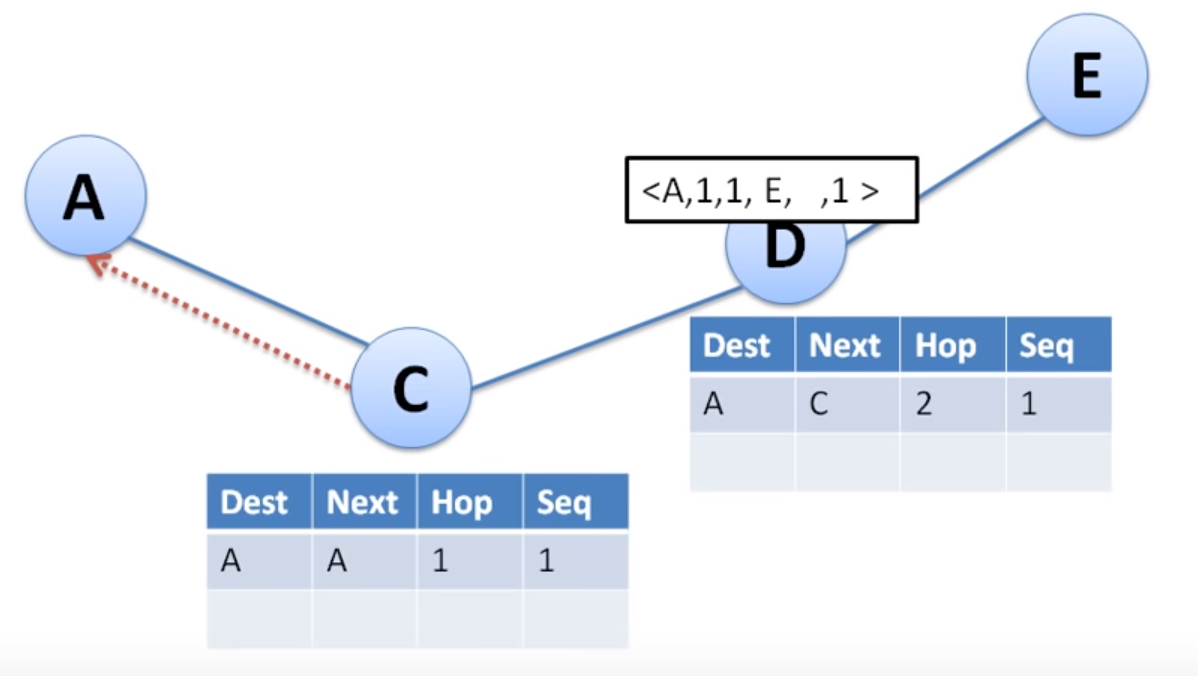
\includegraphics[width=8cm]{handle_route_request_2}
\caption{处理和转发路由请求:2}
\end{figure}

\subsubsection{生成路由回复}
一个节点在以下情况会生成路由回复消息:
\begin{itemize}
	\item 节点本身就是目标节点。
	\item 节点存在到目的节点的一条有效路由,且路由表项内的目的节点序列号有效并且不小于RREQ消息内的目的节点序列号
\end{itemize}

RREP一旦被创建,RREP消息就将被送往通向发起节点的下一跳节点,这个节点由路由表里通向发起节点的路由表项给出。当RREP被转发回发起节点时,“跳数”每一跳都会加一,因此当RREP到达发起节点时,这个跳数应当和发起节点到目的节点的跳数一致。

\begin{figure}[htb]
\centering
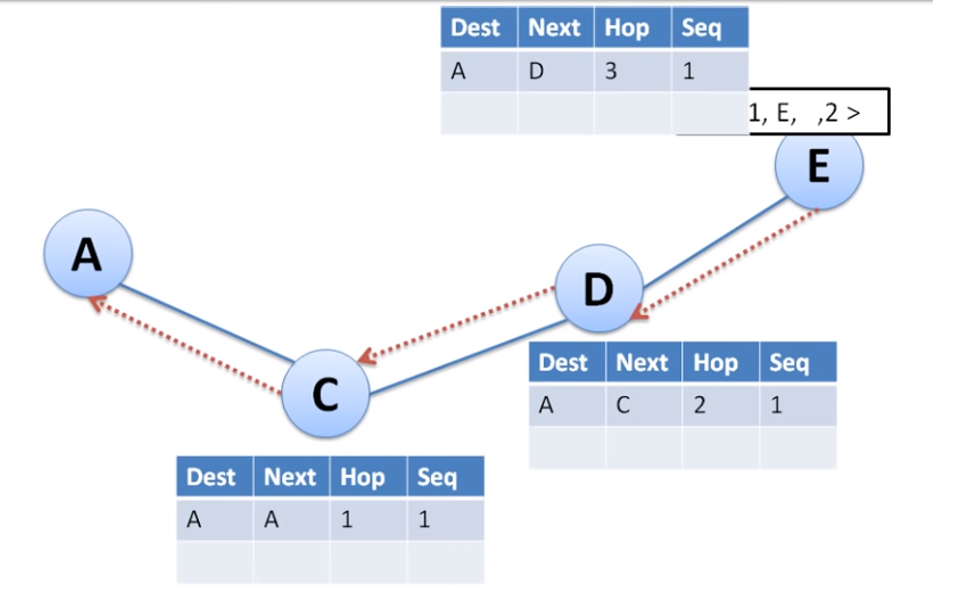
\includegraphics[width=8cm]{gen_route_reply_1}
\caption{生成路由回复:1}
\end{figure}

\begin{figure}[htb]
\centering
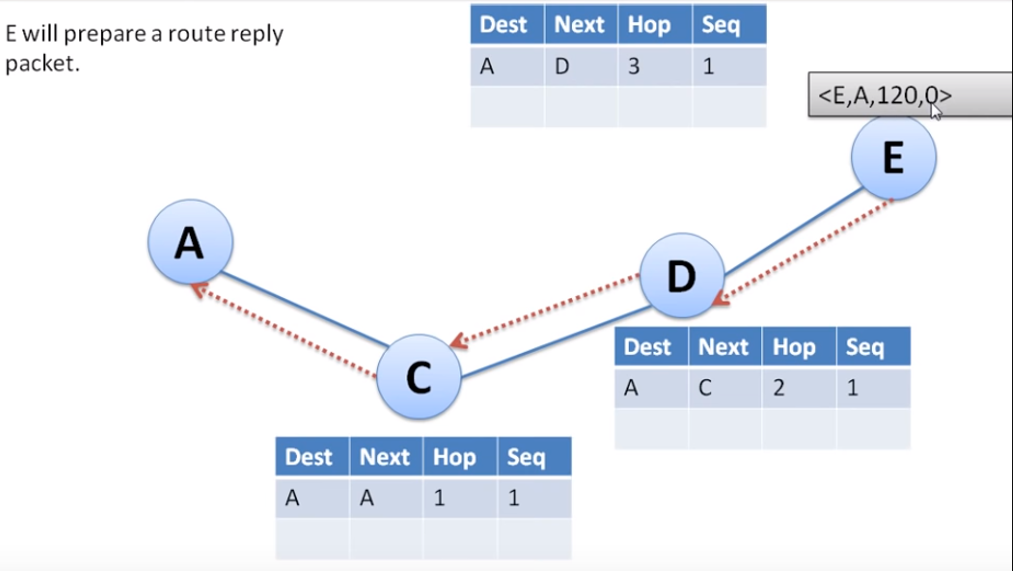
\includegraphics[width=8cm]{gen_route_reply_2}
\caption{生成路由回复:2}
\end{figure}

\subsubsection{接受和转发路由回复}
当一个节点收到RREP消息,它将搜索(使用最长前缀匹配)到前一跳的路由;在RREP转发回源节点的过程中,沿着这条路径上的每一个节点都将建立到目的节点的同向路由,即在路由表中记录下RREP是从哪一个邻居节点传来,然后更新有关源和目的路由的时间信息并记录下RREP中目的节点的最新序列号。对于那些建立了反向路由,但RREP并没有经过的节点,它们建立的反向路由将会在一定时间(Active-Route-Timeout)后自动变为无效。

收到RREP的节点将会对到源节点的第一个RREP进行转发,对于其后收到的到同源的RREP,只有当后到的RREP中具有更高的目的序列号或目的序列号相同但所经过的跳数较少时,节点才会重新更新路由信息并将该RREP转发。根据AODV协议的规定,源节点将在收到第一个RREP后,就开始向目的节点发送数据。

\begin{figure}[htb]
\centering
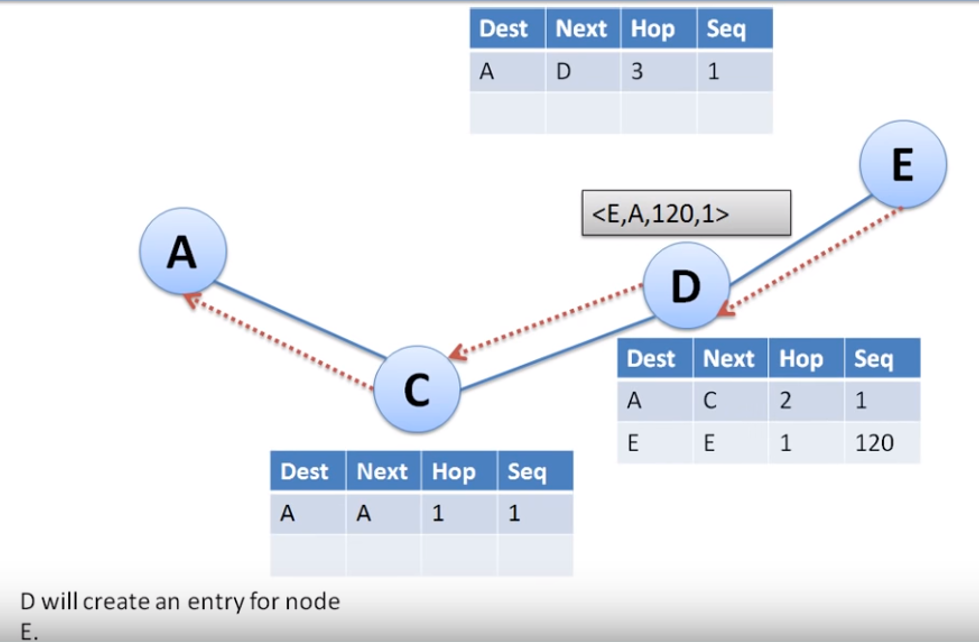
\includegraphics[width=8cm]{receive_route_reply_1}
\caption{接受和转发路由回复:1}
\end{figure}

\begin{figure}[htb]
\centering
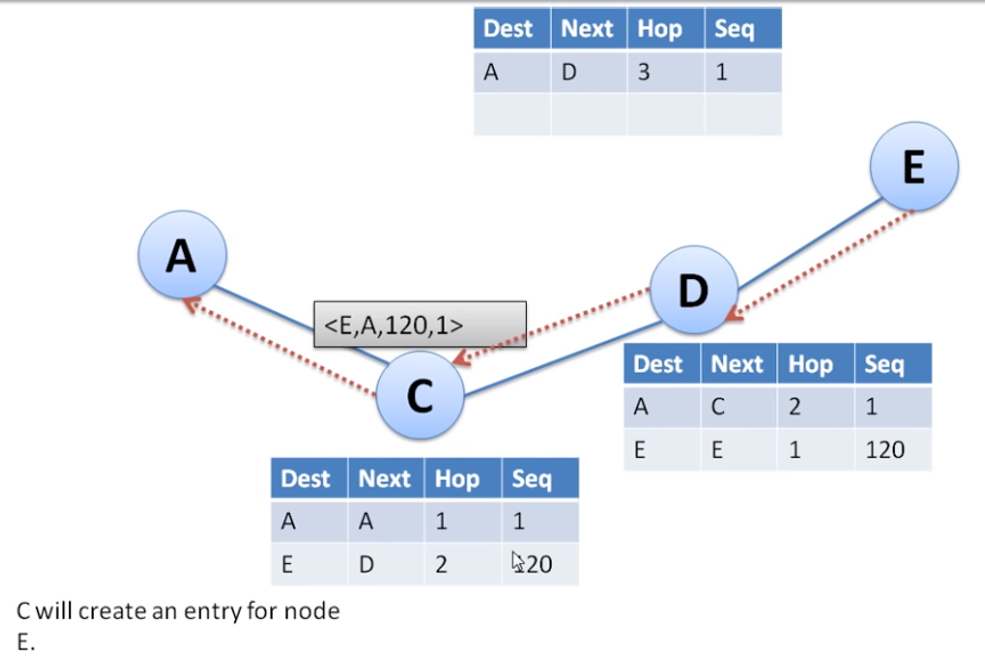
\includegraphics[width=8cm]{receive_route_reply_2}
\caption{接受和转发路由回复:2}
\end{figure}

\begin{figure}[htb]
\centering
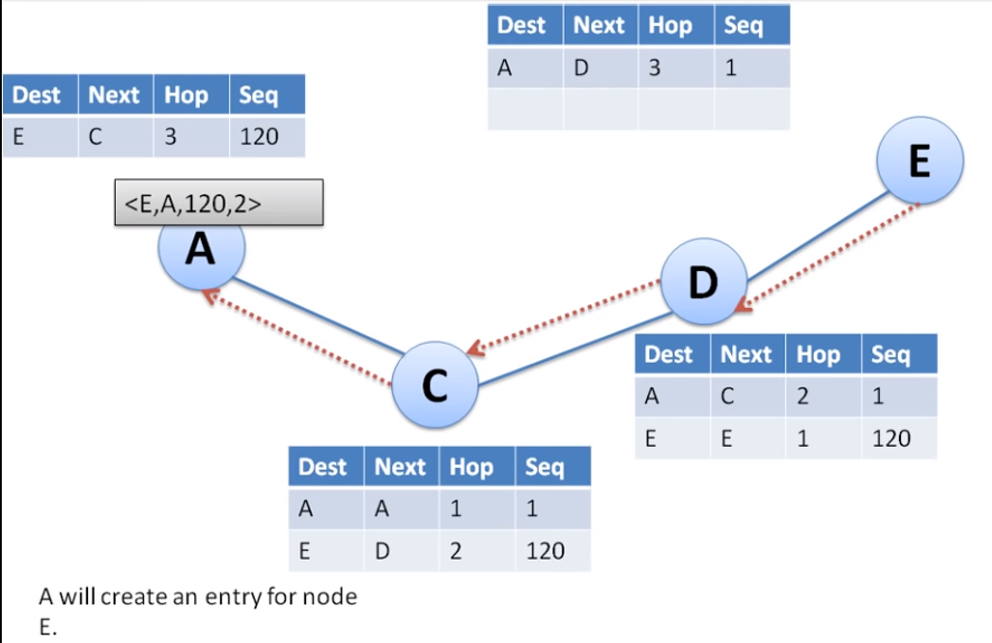
\includegraphics[width=8cm]{receive_route_reply_3}
\caption{接受和转发路由回复:3}
\end{figure}

\clearpage

\section{基于AODV的支付通道网络}
基于对ADOV协议特性的分析,以及反应式路由和主动式路由的比较,我们决定使用反应路由算法,因为它具有获得最新路由、路径无环和快速适应不断变化的网络条件的能力。此外,由于每个节点都可以自行决定支付的方式,因此更容易维持其经济动机。

我们使用无向图来定义PCN支付通道网络$G=(N,C)$,其中$N$是节点的集合,$C$是节点间的通道$C\subseteq \left\{(n_1,\ n_2)\ |\ n_1,\ n_2\in N\right\}$。每个节点$n$代表一个独立的参与方,通过扮演一个积极的支付者或收款者的角色来参与到整个网络中,或者通过作为一个中间节点来被动的赚钱。每个节点都会被分配一个全局惟一的ID。

对于任意$c\in C$, 定义$bal(n,c)$为通道$c$中节点$n$的当前余额的二元函数$Bal: N\times C\rightarrow[0,+\infty)$,当通过通道$c$转发一个支付,一个中间节点$n$可能收取一定的费用$f\in(-\infty,+\infty)$,并提供一个利率$r\in\ [0,+\infty)$。也就意味着,通过一个节点$n_i$发送金额$x$的总费用是$p_i=r_i\times x+f_i$;发送节点必须支付$p_i$,以便$x$可以到达下一个节点,而中间节点将自己扣除$f_i$。因此,从起始节点$n_1$向中间节点$n_2$和$n_3$发送支付的总成本$p$(支付费用)可以表示为$p=p_3(p_2(x))$ 或者$p=r_3\times\left(r_2\times x+f_2\right)+f_3$。

\subsection{路由发现}
按照AODV的RFC设计,只有当节点决定通过网络发送支付时才会发出路由发现,即路由请求被广播到每个连接节点(通过支付通道连接的节点)
每一个路由请求REQ可以以如下的方式表示:
\begin{equation}
REQ=\langle n_o, n_d, n_l, {nr}_d, {nr}_o, d_{req},d_{route},\#_{max},\#_{rate},\#_{fee},\#_{hops}\rangle
\end{equation}
REQ可以分为两部分来理解,一部分对应原始AODV中就有的字段,另一部分则是针对PCN网络的复杂性新增的字段。

\textbf{原始AODV中的字段:}
\begin{itemize}
	\item $n_o$是路由请求的发起者;每个节点都可以通过一个指向$n_o$的路径更新其本地路由表
	\item $n_d$是预期的接收者,即目的节点
	\item $n_l$对应最后一跳的节点;即发送此请求的节点
	\item ${nr}_d, {nr}_o$均是序列号
	\iitem ${nr}_d$:路由发起节点$n_o$在过去收到的通往目的节点的最新序列号
	\iitem ${nr}_o$:用于向路由请求的发起者的路由中使用的序列号
	序列号可以用来反映此路由的新鲜度,一般序列号越大,路由越新鲜,这是保证开环的重要措施,在路由发现和路由应答更新路由时需要进行序列号的比较。
	\item $d_{req}$是请求的生命周期,即该请求的有效期
	\item $\#_{hops}$定义到请求发起者$n_o$的中间节点(跳数)的数量
\end{itemize}

\textbf{为PCN设计的字段:}
\begin{itemize}
\item $d_{route}$定义到$n_o$的有效时间的长度
\item $\#_{rate}$是到达该节点的汇率
\item $\#_{fee}$表示到达该节点的成本费用
\item $\#_{max}$
\end{itemize}

由于每一个通道都有一定的容量限制,因此每个节点通过特定的通道进行支付操作都会有一个确定的最大值,而对于特定节点而言,可能其只愿意转发其中的一部分$\#_{max}$:
\begin{equation}
\#_{max} \leq bal(n_i,c)
\end{equation}
其中$n_i$是通过通道$c$转发此请求的当前节点;该值取决于不同的请求。每当一个节点发出一个请求时,我们就会在每个接收请求的节点上建立一个反向路由(即指向发起节点的路由) ;如果一个节点接收$REQ$,并且不是目的节点,它会在继续发送之前更新$REQ$

\textbf{REQ的更新策略如下:}
\begin{itemize}
\item $n_o, n_d$保持不变
\item $n_l$指向当前节点
\item $\#_{rate}$以其当前的汇率乘以之前的汇率来进行更新,费用也用同样的方法进行更新
\item $\#_{fee}$以当前费用和之前费用的总和来进行更新
\item 当前节点以最后一个$d_{route}$和当前节点愿意将该路由提供给$n_o$的时间之间的最小值来更新$d_{route}$字段
\item 当前节点检查它可以通过通道发送多少金额到$n_l (\#_{maxOld})$,和$n_l$想通过通道发送多少金额$(\#_{maxCur})$,并取这两个值的最小值来计算$\#_{max}$

\begin{equation}
\#_{maxNew}=Min(\#_{maxOld},\#_{maxCur})
\end{equation}
\end{itemize}
因此,使用$REQ$,每个接收节点接收到的信息是,它可以向发起者$n_o(\#_{maxNew})$发送多少信息以及该路由有效的时间是多长。

当一个节点接收到$REQ$时,节点会检查$REQ$是否有效,即检查$d_{req}$是否未过期,以及是否未达到最大跳数;如果$REQ$在遍历时经过比$MAX\_HOPS$更多的中间节点数则请求被丢弃。然后,节点检查是否存在有效通道可以到达最后一跳,以及该通道是否具有足够的余额。为此本地节点将检查它的路由表,查看到达$n_o$的路由是否已经存在,若是如此,节点将检查当前$REQ$是否优于路由表条目,此时本地节点可以遵循自己的经济动机来进行比较(如收取较低的汇率和费用,较长的有效期)。

接着,节点需检查这个请求是否已经被处理过,如果是,则不执行其他操作。检查当前节点是否已经是最终接收方(目的节点);若是如此,将发送$REP$返回到最后一跳$n_l$;同样如果当前节点检查是否已经知晓到达目标节点$n_d$的路由;若是如此,一个$REP$消息将返回到路由表条目中的下一跳。如果当前节点是一个中间节点,则$REQ$ 将被转发与当前节点相连接的所有节点;$REQ$的汇率、费用、$n_l$、$\#_{hops}$都将被更新。由于在$REQ$中节点还承诺了一条通向$n_o$的路径,因此当前节点必须锁定一些资金一段时间;以确保有足够的资金支付通过这条路线。

上述更新策略的伪代码如下:
\begin{figure}[htb]
\centering
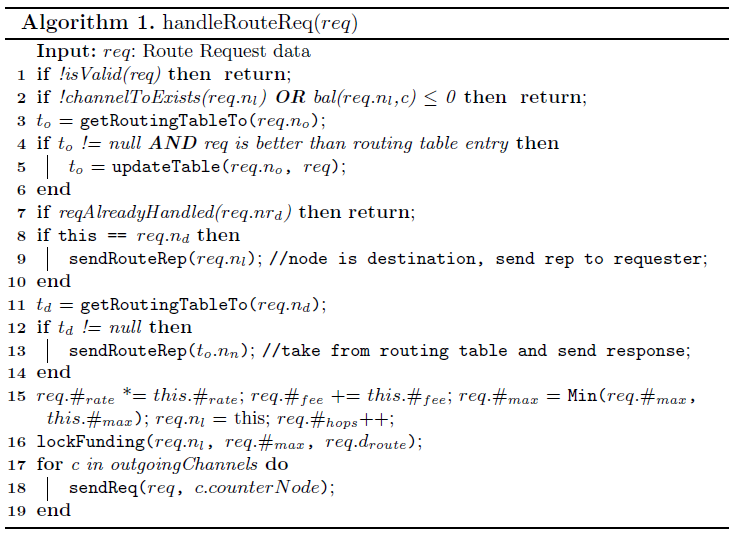
\includegraphics[width=14cm]{req_update}
\caption{$REQ$更新策略}
\end{figure}

\subsection{路由选择}
当$REQ$到达其目标节点$n_d$时,或者如果某个中间节点已经知道通往目标节点的路由,则该路由响应消息($REP$)将返回给发起者
$REP$具有类似于REQ的格式:
\begin{equation}
REP=\langle n_o, n_d, n_l, {nr}_d, {nr}_o, d_{req},d_{route}, \#_{max}, \#_{rate},\#_{fee}\rangle
\end{equation}
$n_o$即它是$REQ$消息的目的节点;$n_d$即$REQ$的发起节点;$n_l$它总是设置为消息发送的最后一跳;${nr}_d,\ {nr}_o$为序列号,前者是路由目标节点的最新序列号,后者是路由请求的发起者$n_o$路由中要使用的序列号
当一个节点接收到了一个$REP$时,节点会先检查通道是否有效,检查是否有足够的可用资金来到完成最后一跳,之后检查本地路由表是否有到达节点$n_o$的路由,以及已知路由是否优于$REP$中的新路由;同样,本地节点可以遵循自己的经济动机,只接受合适的路由。如果新的路由更好,或者路由表条目不存在,路由表将使用一个指向目标节点的新条目更新
相反,如果一个路由已经存在,那么这个过程就在这里结束。

接着会验证当前节点是否就是目标节点,若是如此,则流程在这里结束,本地节点可以沿着这条路径发出付款;或者,当前节点是一个中间节点,用于转发$REP$,为此,它在路由表中检查是否存在通向$n_d$的路由,如果没有找到路由,则无法转发$REP$,进程就此结束;因此,如果到达$n_d$的路径已知,那么将更新$REP$消息,$\#_{max},\#_{rate},\#_{fee},n_l$ 均被更新。
然后,节点锁定承诺路由的最大数量$\#_{max}$,并根据路由表条目将路由转发到下一个节点
与路由发现阶段类似,最重要的部分是在路由有效的时间内锁定特定通道中的资金;由于此信息仅在本地节点中保持脱机状态,因此它仅表示资金可用的承诺,但不能$100\%$保证路由在$d_{route}$过期之前有效。

\begin{figure}[htb]
\centering
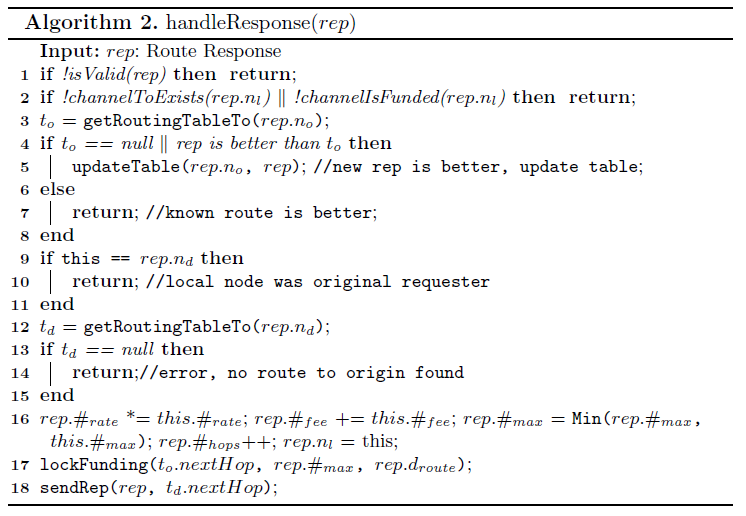
\includegraphics[width=14cm]{select_route}
\caption{路由选择}
\end{figure}

下图显示了从节点A到节点E的路由是如何建立的过程
节点A向其连接的邻居发送路由请求$({REQ}_1)$,如B,B依次将这个请求转发给C和D $({{REQ}_2}_1, {{REQ}_2}_2)$等等,最后,$REQ$到达节点E,该节点返回一条针对发起者A的$REP$消息。由于每个REQ包含如何到达发起者节点的信息,因此本例中的每个节点现在都拥有如何路由到节点A的信息。
于是节点E沿着A的路径发出第一条${REP}_1$消息,消息首先传递节点$D({REP}_1)$,节点$B ({REP}_2)$,最终到达节点$A ({REP}_3)$。
如果节点C现在想要向节点A进行支付操作,它可以立即支付,因为它已经拥有了所有的路由信息。如果C要支付E,只需要向B发出一份要求,B已经知道了需要的信息,并立即退回$REP$。
因此,整个网络越活跃,找到路由所需的传递消息也就越少。

\begin{figure}[htb]
\centering
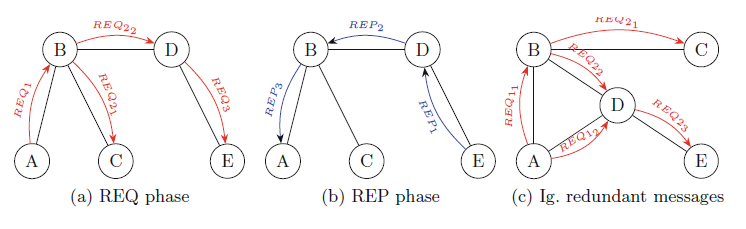
\includegraphics[width=14cm]{create_route}
\caption{\label{create_route} 建立节点A到E的路由}
\end{figure}

\clearpage

\section{评估}
为了明确被修改过的AODV路由协议(例如增加费用和汇率字段来增强消息)是否适用于PCN中的支付路由,作者在模拟环境中对其进行了评估。截至编写论文时,闪电网络刚在比特币主网上线,还没有其大规模使用情况下的实际数据可供参考。因此,作者在本节中对网络拓扑自行做出一些假设。

\subsection{测试环境搭建}
作者使用包含500、1000和5000个节点的三种网络拓扑结构来评估他们的路由协议。网络包含三种区块链,包括BTC、ETH和LTC。每个节点以一个统一的概率$p=0.3$放置在这三个区块链中的一个里。然后,在节点最少的区块链中随机选择若干节点作为流动性提供者,即它们在两个区块链上共有一个钱包,从而得以通过它们进行路由。 三个区块链通过这样的操作两两连接。下一步,根据Watts和Strogatz发表的关于小世界网络的论文,作者随机连接同一链内的节点。

\begin{figure}[htb]
\centering
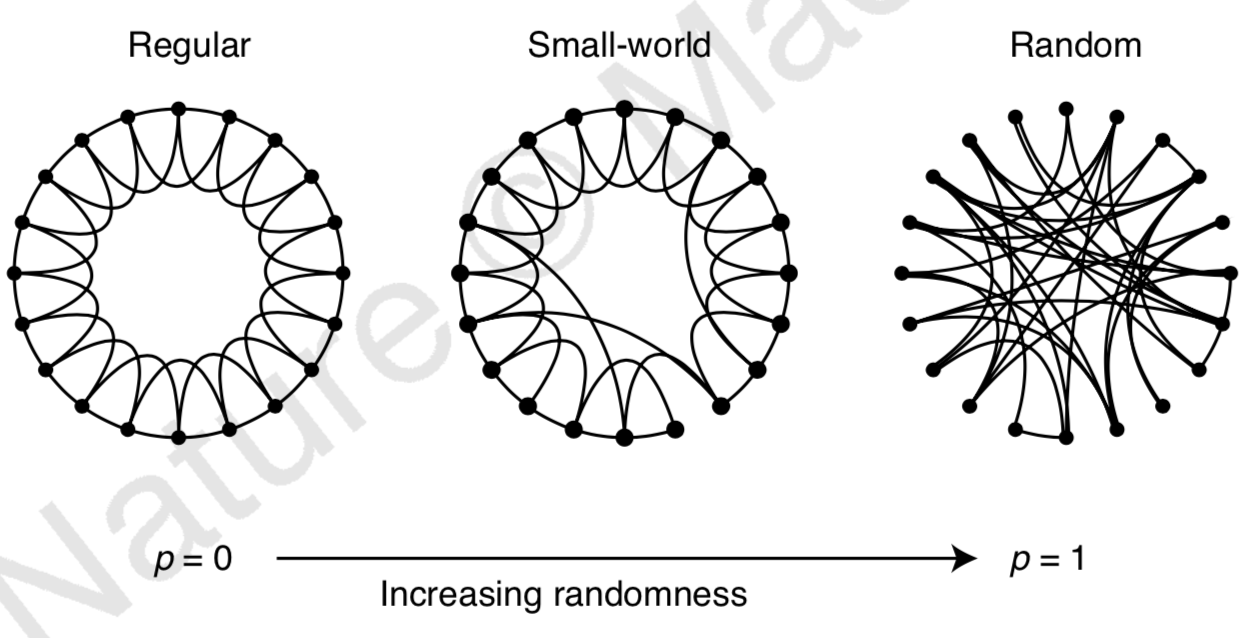
\includegraphics[width=14cm]{image-20181127153048202}
\caption{\label{image-20181127153048202} 三种随机重新连线情况}
\end{figure}

小世界网络的集体动力学这篇论文中提到的连接方法如图\ref{image-20181127153048202}。先将所有的点摆放为如图所示的规则的环形网络,每个顶点由无向边连接到它的k个最近的点,如图\ref{image-20181127153048202}中 $k=4$。然后选择一个顶点,考虑连接到顺时针最近点的边,以概率$p$重新连接到环上随机点,如果出现重复的边则不连接。顺时针依次选择顶点,重复上一步骤,直到绕完一圈。然后考虑连接到顺时针第二近点的边并以概率$p$重新连接到环上随机点,如果出现重复的边则不连接。顺时针依次选择顶点,重复上一步骤,绕完一圈。重复以上步骤,直到原始图的所有边都被考虑过一次。整体看来,因为在整个图中有$\frac{nk}{2}$条边,所以$k/2$圈后重新连线过程结束\cite{watts1998collective}。

为什么要这么连线呢?我们翻阅了一定数量的论文,没有看到太多解释,只能暂时理解为这样处理所建立的特殊网络模型(叫做WS模型)恰好符合现实生活中的许多案例(如电影演员合作网、电力网、线虫、人际关系网络、脑神经网络、公路交通网络)的特性,即顶点数$n$远大于平均连接数k远大于$ln(n)$远大于1。其中k远大于$ln(n)$是为了保证网络不会稀疏到失去连通性\cite{bollaba1985random},用通俗的语言来说,就是在一个由大量节点组成的网络中,大部分的节点彼此并不相连,但绝大部分节点之间经过少数几步即可到达。这样的特性,和PCN也是比较符合的。

作者设置每个节点的链内平均连接数$k=4$,重新连线的概率$p=0.3$。作者使用了GitHub上的开源项目Watts Strogatz Generagtor\cite{gs-ui-swing}来生成这样的图。每个通道两侧的资金随机设置为$[1,100]$。这里忽略了现金单位,也就是说一个通道最多拥有BTC数:$MAX(bal(c))=200$,最少拥有$MIN(bal(c))=2$ LTC。三种币之间的汇率从网站\cite{coin_market_cap}上查询并采用固定值,即1 ETH = 0.07508560 BTC,1 LTC = 0.01262120 BTC,1 LTC=0.16506884 ETH。每个流动性提供者提供相同的汇率。每个节点在转发付款时随机收取的费用也为固定值,值在$[0,1]*10^{-9}​$中随机取得。生成的拓扑的详细信息可在表1中找到。注意,由于通道是双向的,两个节点之间的连接记为一个通道。

\begin{figure}[htb]
\centering
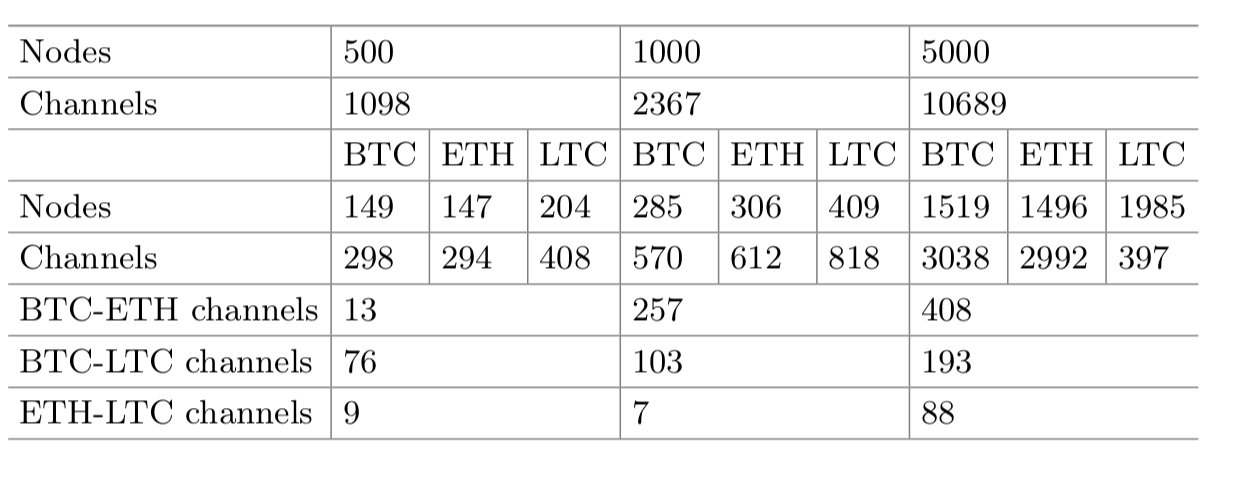
\includegraphics[width=14cm]{image-20181127153012674}
\caption{测试设置}
\end{figure}

\subsection{测试方案}
为了验证这个路由协议,作者在每个网络拓扑上运行了1000次随机生成的交易,即随机选择一个节点向另一个节点支付。支付金额在$[0,1]*10^{-9}$间随机生成。注意,虽然理论上可能有更小的支付金额以至于无法立即记录这笔支付而且我们因此不限制这一点,但实际上这应当需要一个不一样的配置。这意味着,如果一次支付是1/10的币,我们需要10次这样的支付才能得到一个能注意到的变化,因此,作者忽略了这个因素。AODV路由协议的限制因素是跳数,即当$REQ$已遍历超过$MAX\_HOPS$个中间节点,这个请求会被丢弃。因此,我们使用不同的$MAX\_HOP$运行每个交易,$MAX\_HOP=[0,N]$,其中N对应于最便宜的可能路径,但是上限为10。换句话说,如果两个节点直接连接则跳数为0且他们之间有一个通道。如果他们中间有一个节点,则跳数为1并且他们之间有两个通道。因此,一次交易最多有10跳或11个通道。最便宜的可能路径由Floyd-Warshell所有节点对最短路径算法手动计算。由于单个路由请求可能改变网络拓扑,我们在每次新请求前会重置节点和通道状态。我们比较了找到的路径与最优路径,即每个跳数下的最便宜路径。这意味着较低的跳数可能导致比最优路径更贵的路径。此外,我们统计了发送的全部信息并测量可达性,即各跳数下有多少成功交易。

\subsection{测试结果分析}

\begin{figure}[htb]
\centering
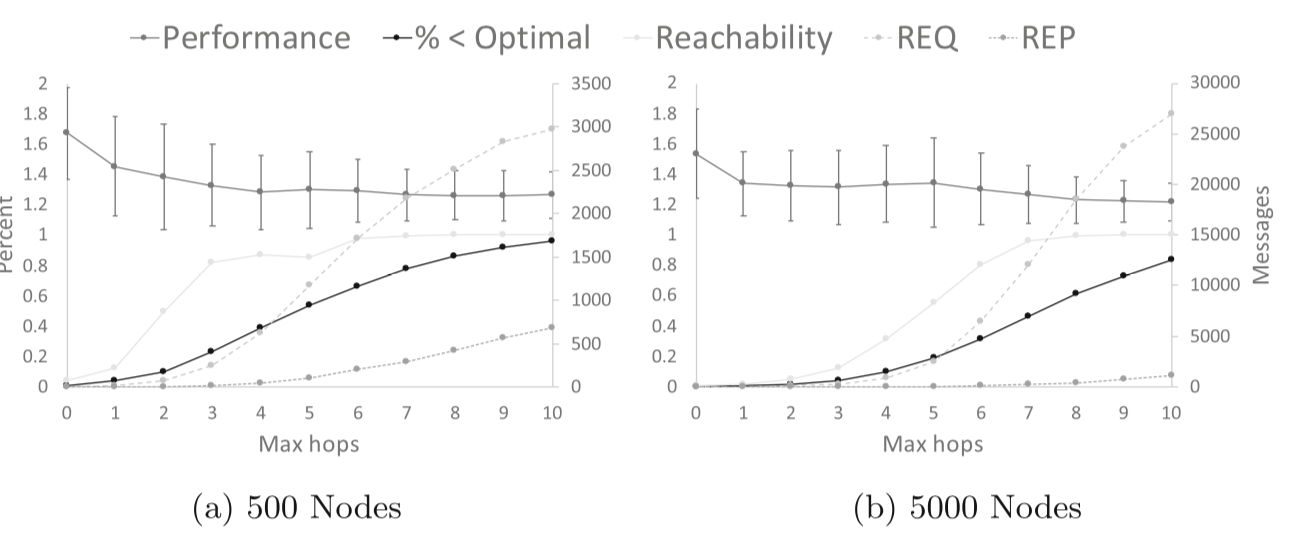
\includegraphics[width=14cm]{image-20181127161041797}
\caption{\label{image-20181127161041797} 测试结果}
\end{figure}

测试结果可以在图\ref{image-20181127161041797}上找到(由于空间有限,没有显示1000个节点的情景)。如之前所提到的,我们有3个不同的网络拓扑结构,分别有500、1000和5000个节点。在每个拓扑上,我们运行了1000次随机选择的交易,即付款人和收款人是随机选择的。每次交易都运行N+1次,其中N的上限为10或者最优路径的跳数。如果两个节点之间存在中间节点,则它们之间需要一跳,如果他们直接连接,则需要0跳。$\overline P$是性能$P$的算术平均值。它表示找到的路径比最优路径平均贵多少。例如$\overline P$值为1.53表示找到的路径的费用平均为最优路径的1.53倍。另外,$\sigma_{\overline P}$表示$\overline P$的标准方差。为简单起见,我们通过除以交易数来将$REQ$和$REP$的消息数量正则化。

如图所示,随着$MAX\_HOP$越大,性能$\overline P$慢慢接近1。$MAX\_HOP$到10的时候$\overline P$没有到1的原因有两方面。

第一个原因,我们允许最大10跳,而有些交易的最优路径超过10跳,这种情况在 500个中有3.9\%,在1000个节点中有1.6\%,在5000个节点中有16.3\%。此外,$\sigma_{\overline P}$随着跳数降低。因此,我们可以说我们的路由找到了更多更接近于实际最优路径的结果。根据跳数,能够找到最优路径的机会由$\%<Optimal$表示。可以看出,跳数越大,找到最优路径的机会越大。

第二个原因是,尽管最大跳数满足条件,还是有可能永远找不到最优路径。这可以归结为作者试图保持不必要的信息较少的原因。具体来说,除非信息更新或更好,否则每个节点只处理一次REQ和REP。图1c展示了一次从A到E的路由请求。在第一阶段,A向B和D($REQ_{1_1}$和$REQ_{1_2}$)。一收到,这些节点就会继续向前转发,B向C和D发送$REQ_{2_1}$和$REQ_{2_2}$,D向E发送$REQ_{2_3}$。因为D已经从A收到了A到E的支付$REQ$,它会忽略来自B的这条消息。未考虑从A经过B到D的路径比A到D便宜,可能成为取得最优路径的限制因素。但是我们为了减少REQ的总量而刻意这样,否则网络可能会被完全淹没。此外,为了更有可能找到更好的路线,我们允许以下情况。如果来自B的$REQ$到达D时,D已经找到了D到E的一条路径,D会返回一条$REP$。因此在这种情况下,A将接受两条$REP$,并可以从中选择较优路径。这解释了为什么我们的测试结果中有较多的$REP$。这些图展示了用交易发送量正交化的$REQ$和$REP$总量。显然,随着允许跳数的增加,$REQ$和$REP$的总量几乎成指数增长。问题在于每个节点正在处理的信息,即,当忽略已经处理的$REQ$信息时,它不知道是否有一个节点从另一个节点中接收了这个信息。一个简单的解决方法是在$REQ/REP$中加入它到达过的节点的信息。但是,虽然这样可以减少消息总量,但是这样将会增大消息的尺寸大小。

有趣的是,对于500节点和1000节点,我们可以达到9\%的可达性,但是对于5000节点,只需要7跳就能达到相似的可达性。最大跳数的增加导致$REQ$数量急剧增加,当允许6跳时有80\%的可达性并产生6405条$REQ$,当允许7跳时有98\%的可达性并产生12097 条$REQ$。因此,作者建议为最大允许跳数设置动态值,即当网络增长时最大跳数增加。注意,随着节点缓存路由信息一段时间后,$REQ$的总量随着时间大幅下降。在图\ref{create_route}的例子中,最初A想要支付给E时,至少有5条$REQ$被广播。但B稍后想要支付给E时,它可能已经有需要的信息,不需要发送$REQ$就可以立即执行支付。

虽然数据显示针对线下网络支付路由修改的AODV对于高达几千名参与者的网络来说是完全可行的,但我们怀疑它是否能扩展到数百万的用户。与AODV中一样,消息大小相对较小(~80 bytes),网络应该能轻松地同时处理几千个请求(加起来仅几兆字节)。虽然已建立的路由可能会随时间的推移而过期,但使用路由维护信息就可以更新关键信息。原始路由请求发出者会沿所需路由发送维护消息,每个中间节点用其当前的交易费用和其通道中的资金分布来更新信息,并将消息沿路径继续转发。因此,一旦一条路径建立起来,只要定期更新,就可以无限重用。

\subsection{安全性分析}
与Flare相比,作者基于AODV的协议不考虑对消息及其内容进行安全保护。因此,发送者和接收者可能在支付路径上被公开。但是,在保护AODV路由协议上研究人员也做了大量尝试。为了提高安全性,过去已经提出了AODV的多种扩展:例如SAODV或 ARAN使用数字签名和哈希链来验证消息的非可变字段和可变信息。这些扩展可以防止控制消息的篡改和数据丢弃攻击。但作者认为,数据篡改的保护不是必要的,因为路由执行遵循原子原则,即所有的交易要么都成功要么都失败,不会存在交了一半钱的情况。这意味着,如果一个中间节点在费用上说了谎,稍后支付将会失败,因为发送者仅只附加了足够让期望的金额到达接收者的钱,如果中间节点多收取了交易费用就会交易失败。隐私和匿名一直是集成了洋葱路由的Flare关注的问题,只有接收者实际知道谁发送给了谁,所有中间节点只是将其转发给下一跳。这样的系统的确更加私密,但是已表明在每个节点以类似的时间帧将将交易广播到区块链的情况下,可以从整个网络中推断路径的线索。更重要的是,在源路由汇总,边缘节点可以滥用这种匿名性来攻击中间节点,使其无法转发支付。为此,攻击者需要在一个或几个节点上分布有比受害者更多的资金,并需要能控制收款人。攻击者通过中间节点发起支付请求,使其需要锁住资金一段时间。当支付失败时锁定会自动释放。但同时这个节点也不能将资金用于其他目的,例如参与其他支付流程并无法通过额外的费用赚钱。使用AODV可以完成同样的攻击。但不同之处在于,在AODV中每个发送者对于中间节点是已知的,这和使用洋葱网络后发送者和接收者保持匿名性不同。因此,使用AODV,每个节点都可以通过接受或拒绝特定节点的路由请求来保护自己。

最后但同样重要的是,去中心化的路由的一个普遍问题是需要每个参与节点在线,因为离线节点不能转发任何请求。这就是为什么闪电网络(或其他支付通道网络)通过赚取路由支付的交易费用来鼓励节点保持在线。

\subsection{小结}
本节我们介绍了基于AODV的支付通道路由协议的功能及性能测试。实验用费用和汇率增强了信息,以找到经济的路线。AODV是一种被动路由协议,仅在需要时建立路由,从而避免了主动路由协议中发送大量信息的开销。但是,如果未征求设置最大跳数,AODV有淹没网络的风险。作者的实验表明经过调整的AODV能轻松地用于多达几千个节点的网络中。因此基于AODV的路由协议可以集成到PCN中。在未来的工作中,作者将重点关注可进一步扩展的路由协议,并评估节点的费用管理如何影响流动性。在各自的开发商中,有限制的流动性是链下通道网络一个众所周知的有待解决的问题。

\clearpage
\section{总结与展望}
本文以基于AODV的支付通道路由协议的必要性、原理、设计以及测试为主要内容展开,并概括介绍了区块链的现状及问题,PCN的提出及问题,几种适用于移动自主网络的路由协议对比及应用于PCN的Flare协议。本篇报告的撰写过程中,我们几位组员分工合作,有效地扩展了对区块链及PCN的认知。我们感受到区块链的优势和潜力无限,未来必定会应用到更多的领域中,而此次报告也将成为我们深入学习领域知识,深入研究原理及应用的开端。

\clearpage
\bibliographystyle{IEEEtran}
\bibliography{ref}

\end{document}